\section{Formulario}
    \subsection{Trigonometria}\label{Trigonometria}
        \begin{enumerate}
            \item {
                $\sin^2(\alpha) + \cos^2(\alpha) = 1$
            }
            \item {
                $\cos(\alpha)=\pm\frac{1}{\sqrt{1+\tan^2(\alpha)}}$
            }
            \item {
                $\sin(\alpha)=\pm\frac{\tan(\alpha)}{\sqrt{1+\tan^2(\alpha)}}$
            }
            \item {
                $sinc(\alpha)\triangleq\frac{\sin(\pi\alpha)}{\pi\alpha}$ 
                É un $\sin(\alpha)$ smorzato secondo $\frac{1}{x}$ che si annulla in $k\pi: k\in\mathbb{Z}$
                \begin{figure}[H]
                    \centering
                    \begin{tikzpicture}
                        \begin{axis}[
                            domain=-6:6,
                            samples=200,
                            axis lines=middle,
                            xlabel=$x$,
                            ylabel=$y$,
                            ymin=-1.5,
                            ymax=1.5,
                            xtick={-5,-4,-3,-2,-1,0,1,2,3,4,5},
                            xticklabels={$-5$,$-4$,$-3$,$-2$,$-1$,$0$,$1$,$2$,$3$,$4$,$5$},
                            ytick={-1, 1},
                            yticklabels={$-1$, $1$},
                            width=12cm,
                            height=6cm
                        ]
                        \addplot [blue, thick] {sin(deg(x*pi))/(x*pi)};
                        \end{axis}
                    \end{tikzpicture}
                    \caption{grafico $sinc(\alpha)$}
                    \label{fig:grafico sinc}
                \end{figure}
            }
        \end{enumerate}
        \subsubsection{Formule di addizione}\label{Trigonometria_Addizione}
            \begin{enumerate}
                \item {
                    $\cos(\alpha \pm \beta) = \cos(\alpha)\cos(\beta) \mp \sin(\alpha)\sin(\beta)$
                }
                \item {
                    $\sin(\alpha \pm \beta) = \sin(\alpha)\cos(\beta) \pm \sin(\beta)\cos(\alpha)$
                }
                \item {
                    $\tan(\alpha \pm \beta) = \frac{\tan(\alpha) \pm \tan(\beta)}{1 \mp \tan(\alpha)\tan(\beta)} $
                }
            \end{enumerate}
        \subsubsection{Formule di duplicazione}\label{Trigonometria_Duplicazione}
            \begin{enumerate}
                \item {
                    $\sin(2\alpha) =2\sin(\alpha)\cos(\alpha)$ 
                }
                \item {
                    $
                        \cos(2\alpha)
                        \begin{cases}
                            \cos^2(\alpha) - \sin^2(\alpha) \\
                            2\cos^2(\alpha)-1\\
                            1-2\sin^2(\alpha)
                        \end{cases}
                    $
                }
                \item {
                    $\tan(2\alpha) =\frac{2\tan(\alpha)}{1-\tan^2(\alpha)}$ 
                }
            \end{enumerate}
            \subsubsection{Formule di bisezione}\label{Trigonometria_Bisezione}
                \begin{enumerate}
                    \item {
                        $\sin(\frac{\alpha}{2}) =\pm\sqrt{\frac{1-\cos(\alpha)}{2}}$ 
                    }
                    \item {
                        $\cos(\frac{\alpha}{2}) =\pm\sqrt{\frac{1+\cos(\alpha)}{2}}$ 
                    }
                    \item {
                        $
                            \tan(\frac{\alpha}{2})
                            \begin{cases}
                                \sqrt{\frac{1-\cos(\alpha)}{1+\cos(\alpha)}} \\
                                \frac{1-\cos(\alpha)}{\sin(\alpha)}\\
                                \frac{\sin(\alpha)}{1+\cos(\alpha)}
                            \end{cases}
                        $
                    }
                \end{enumerate}
    \subsection{Segnali Notevoli}\label{Segnali Notevoli}
    \begin{enumerate}
        \item {
            $x_R\triangleq A\hspace{0.1cm}rect\left(\frac{t}{T}\right)\hspace{0.7cm} T = durata $
                \begin{figure}[H]
                    \centering
                    \begin{tikzpicture}
                        \begin{axis}[
                            xlabel=$x$,
                            ylabel=$y$,
                            xmin=-5,
                            xmax=5,
                            ymin=-0.5,
                            ymax=4,
                            ytick = {1.5},
                            xtick={-3,-1.5, 0, 1.5,3},
                            xticklabels={$-\frac{T_0}{2}$,$-\frac{T}{2}$, $0$, $\frac{T}{2}$, $\frac{T_0}{2}$},
                            yticklabels = {$A$},
                            yticklabel style = {yshift=5pt,xshift=4pt}, 
                            axis lines=middle,
                            thick,
                            domain=-5:5,
                            samples=100,
                            width=10cm,
                            height=4cm
                        ]
                        \addplot [const plot,red, thick] coordinates{(-1.5,1.5)(1.5,1.5)};
                        \addplot [const plot,red, thick] coordinates{(-1.5,0)(-1.5,1.5)};
                        \addplot [const plot,red, thick] coordinates{(1.5,0)(1.5,1.5)};
                        \addplot [const plot,red, thick] coordinates{(5,0)(1.5,0)};
                        \addplot [const plot,red, thick] coordinates{(-5,0)(-1.5,0)};
                        \end{axis}
                      \end{tikzpicture}
                    \caption{Rappresentazione di $A\hspace{0.1cm}rect\left(\frac{t}{T}\right)$}
                    \label{fig:grafico rect}
            \end{figure}                
        }
        \item {
            $sinc(\alpha)\triangleq\frac{\sin(\pi\alpha)}{\pi\alpha}$\\ 
            É un $\sin(\alpha)$ smorzato secondo $\frac{1}{x}$ che si annulla in $k\pi: k\in\mathbb{Z}$
            \begin{figure}[H]
                \centering
                \begin{tikzpicture}
                    \begin{axis}[
                        domain=-6:6,
                        samples=200,
                        axis lines=middle,
                        xlabel=$x$,
                        ylabel=$y$,
                        ymin=-1.5,
                        ymax=1.5,
                        xtick={-5,-4,-3,-2,-1,0,1,2,3,4,5},
                        xticklabels={$-5$,$-4$,$-3$,$-2$,$-1$,$0$,$1$,$2$,$3$,$4$,$5$},
                        ytick={-1, 1},
                        yticklabels={$-1$, $1$},
                        width=12cm,
                        height=6cm
                    ]
                    \addplot [blue, thick] {sin(deg(x*pi))/(x*pi)};
                    \end{axis}
                \end{tikzpicture}
                \caption{grafico $sinc(\alpha)$}
                \label{fig:grafico sinc2}
            \end{figure}
            La banda di una sinc é l'intervallo in cui si annulla $[-\frac{1}{T},\frac{1}{T}]$,es: se $banda\ =1\ se\ T=1$
            \begin{figure}[H]
                \centering
                \begin{tikzpicture}
                    \begin{axis}[
                        domain=-4:4,
                        samples=200,
                        axis lines=middle,
                        xlabel=$x$,
                        ymin=-0.2,
                        ymax=0.2,
                        xtick={-2,0,2},
                        xticklabels={$-\frac{1}{T}$,$0$,$\frac{1}{T}$},
                        ytick={},
                        width=10cm,
                        height=4cm
                    ]
                    \addplot [const plot,red, thick] coordinates{(-2,0)(2,0)};
                    \end{axis}
                \end{tikzpicture}
                \caption{banda}
                \label{fig:banda sinc}
            \end{figure} 
        }
        \item {
        }
        \item {
        }
    \end{enumerate}
    \subsection{Grandezze Fisiche}\label{Grandezze Fisiche}
        \begin{itemize}
            \item {Hertz}
        \end{itemize}

    \subsection{Varie}\label{Varie}
        \begin{itemize}
            \item {
                Calcolo della TCF su MATLAB:\\
                $X_{(f)} = \int_{-\infty}^{\infty} x_{(t)} e^{-j2\pi ft } dt$

                MATLAB calcola un'approssimazione dell'integrale della TCF con un periodo $T$:
                \begin{figure}[H]
                    \centering
                    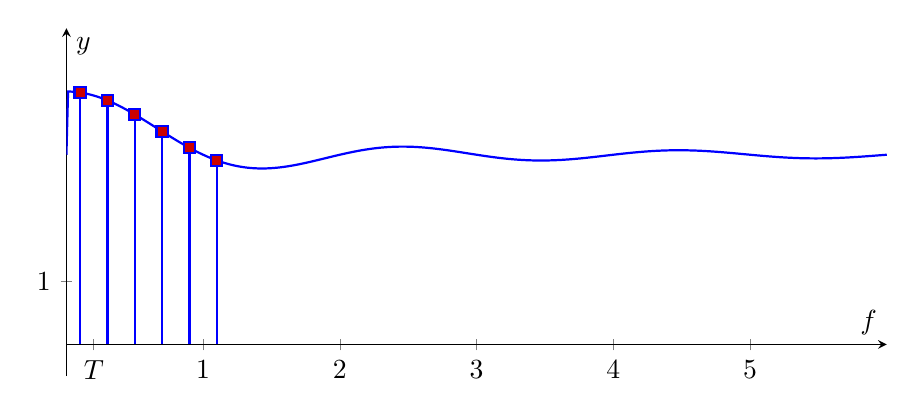
\begin{tikzpicture}
                        \begin{axis}[
                            domain=0:6,
                            samples=300,
                            axis lines=middle,
                            xlabel=$f$,
                            ylabel=$y$,
                            ymin=-0.5,
                            ymax=5,
                            xtick={0,0.2,1,2,3,4,5},
                            xticklabels={$0$,$T$,$1$,$2$,$3$,$4$,$5$},
                            ytick={1},
                            yticklabels={$1$},
                            width=12cm,
                            height=6cm
                        ]
                        \addplot [blue, thick,samples = 500] {(sin(deg(x*pi))/(x*pi))+3};
                        \addplot+ [ycomb,blue, thick, samples at = {0.1,0.3,0.5,0.7,0.9,1.1}] {(sin(deg(x*pi))/(x*pi))+3};
                        \end{axis}
                    \end{tikzpicture}
                    \caption{Campionamento MATLAB}
                    \label{fig:campionamento MATLAB xt}
                \end{figure}    
                \[
                    X_{(f)} = \sum_{n} x_{(nT)}e^{-j2\pi fnT}T
                \]
                Ma nella $f$ é una variabile continua, quindi a sua volta bisogna variare $f$:\\
                \[X_{(fk)} =X_{(k\Delta f)} = \sum_{n} x_{(nT)}e^{-j2\pi \Delta fnT}T\]
                e la condizione sul $\Delta f$ é che $\Delta f<<BB$.
                \begin{figure}[H]
                    \centering
                    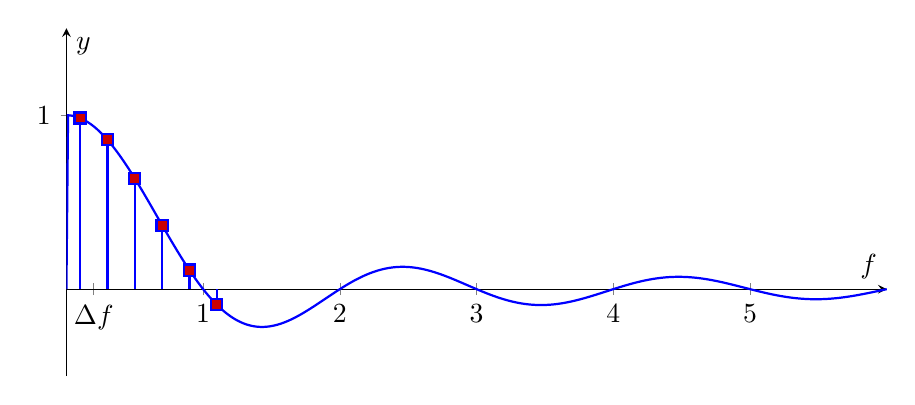
\begin{tikzpicture}
                        \begin{axis}[
                            domain=0:6,
                            samples=300,
                            axis lines=middle,
                            xlabel=$f$,
                            ylabel=$y$,
                            ymin=-0.5,
                            ymax=1.5,
                            xtick={0,0.2,1,2,3,4,5},
                            xticklabels={$0$,$\Delta f$,$1$,$2$,$3$,$4$,$5$},
                            ytick={1},
                            yticklabels={$1$},
                            width=12cm,
                            height=6cm
                        ]
                        \addplot [blue, thick,samples = 500] {sin(deg(x*pi))/(x*pi)};
                        \addplot+ [ycomb,blue, thick, samples at = {0.1,0.3,0.5,0.7,0.9,1.1}] {sin(deg(x*pi))/(x*pi)};
                        \end{axis}
                    \end{tikzpicture}
                    \caption{ $\Delta f$}
                    \label{fig:campionamento MATLAB sinc}
                \end{figure}
            }

        \end{itemize}

    
